\title{Développement}
\subtitle{}
\author{}
\institute{}
\date{}
\begin{frame}
	\maketitle
\end{frame}

\begin{frame}
	\frametitle{Développement}
	\framesubtitle{Séparation vue-modèle}
	\textbf{Avantages}
	\begin{itemize}
		\item Débogage
		\item Modularité
		\begin{itemize}
			\item Séparation des threads
			\item Travail en équipe
		\end{itemize}
	\end{itemize}

	\textbf{Inconvéniants}
	\begin{itemize}
		\item Vite limitant
		\item Difficile à maintenir
	\end{itemize}
\end{frame}

\begin{frame}
	\frametitle{Développement}
	\framesubtitle{Multithreading}

	\textbf{Pourquoi ?}
	\begin{itemize}
		\item Algorithmes longs
		\item Généricité IA-Joueur
		\item Pas de gain de performance (GIL)
	\end{itemize}
	\textbf{Comment ?}
	\begin{itemize}
		\item Machines à état
		\item Ownership pattern
	\end{itemize}
\end{frame}

\begin{frame}
	\frametitle{Développement}
	\framesubtitle{Intelligence artificielle}

	\begin{itemize}
		\item Orienté Objet
		\item Une seule méthode à surcharger
		\item Pas à se soucier des threads
	\end{itemize}

	\begin{figure}[b]
		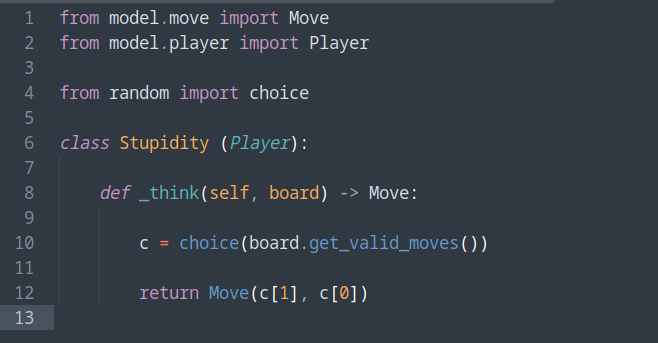
\includegraphics[width=0.7\textwidth]{img/stupidity.png}
		\caption{Code intégral de l'IA "stupidity"}
	\end{figure}
\end{frame}

\begin{frame}
	\frametitle{Développement}
	\framesubtitle{Base de données}

	\begin{figure}
		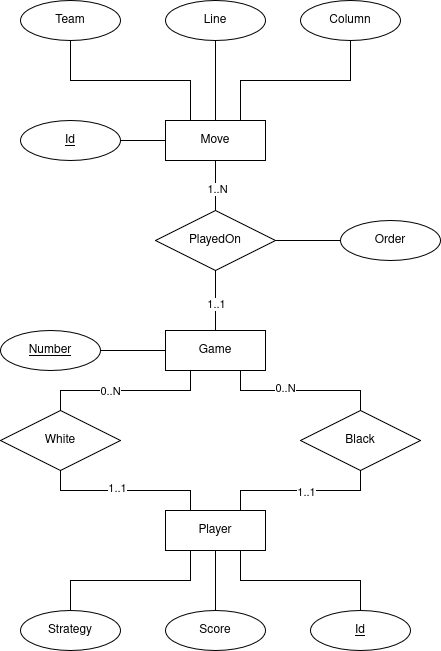
\includegraphics[width=0.4\textwidth]{img/entity_relationship.png}
		\caption{Modèl entité-relation de notre base de données}
	\end{figure}
\end{frame}

\begin{frame}
	\frametitle{Développement}
	\framesubtitle{Base de données}
	\begin{figure}
		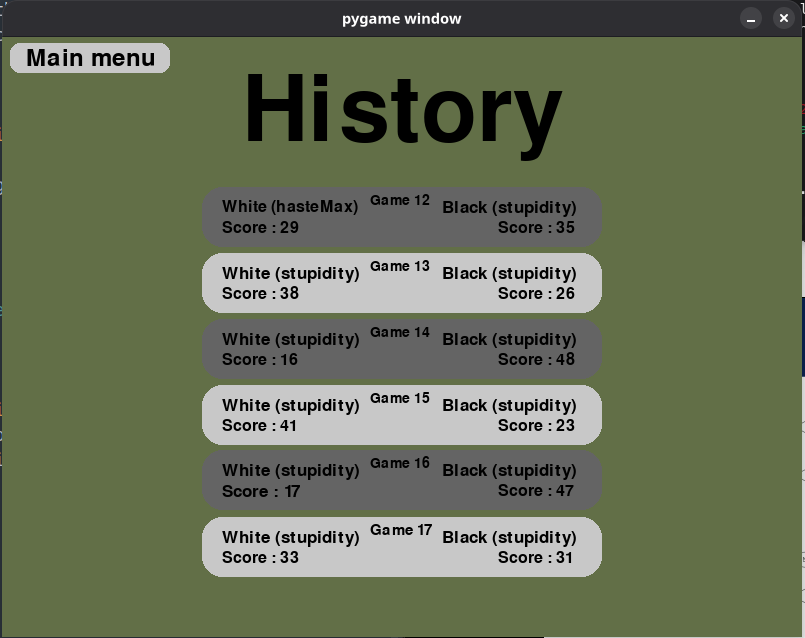
\includegraphics[width=0.7\textwidth]{img/history.png}
		\caption{Affichage dans l'application}
	\end{figure}
\end{frame}